\documentclass{beamer} 
\usepackage{amsmath,amsthm}
\usepackage{graphicx,microtype,parskip}
\usepackage{caption,subcaption,multirow}
\usepackage{attrib}

\frenchspacing

\usetheme{default}
\usecolortheme{whale}

\setbeamertemplate{navigation symbols}{}
\setbeamertemplate{footline}[frame number]

\setbeamercolor{title}{fg=blue,bg=white}

\setbeamercolor{block title}{fg=white,bg=gray}
\setbeamercolor{block body}{fg=black,bg=lightgray}

\setbeamercolor{block title alerted}{fg=white,bg=darkgray}
\setbeamercolor{block body alerted}{fg=black,bg=lightgray}


\AtBeginSection[]
{
  \begin{frame}
    \tableofcontents[currentsection]
  \end{frame}
}

\title{Spring 2016 committee meeting for Peter Smits}
\author{}
\institute{}
\date{}


\begin{document}

\begin{frame}
  \maketitle
\end{frame}

\begin{frame}
  \tableofcontents
\end{frame}


\section{How macroecology affects macroevolution: the interplay between extinction intensity and trait-dependent extinction in brachiopods.}

\begin{frame}
  \begin{alertblock}{Question and analysis}
    \begin{itemize}
      \item How do the effect of emergent traits on duration (\alert{extinction selectivity}) vary with expected duration (\alert{extinction intensity}) and each other?
      \item What is the relationship between environmental affinity and duration wrt specialists versus generalists?
      \item \textbf{Approach:} hierarchical Bayesian survival model, \\varying intercepts and slopes, Weibull distribution, \\imputed gap statistic for taxa with duration \(< 3\).
    \end{itemize}
  \end{alertblock}
\end{frame}

\begin{frame}
  \frametitle{Analysis of post-Cambrian Paleozoic brachiopod genus durations}
  \begin{itemize}
    \item stage as time unit; duration measured in stages
    \item multiple emergent traits analyzed
      \begin{itemize}
        \item geographic range
          \begin{itemize}
            \item used JADE to handle effect of biased sampling \\(Chao et al. 2015 \textit{Ecology})
          \end{itemize}
        \item body size
          \begin{itemize}
            \item from Payne et al from the \textit{Treatise}
          \end{itemize}
        \item environmental preference (x, x\(^2\))
        \item gap statistic as measure of sampling (Foote and Raup 1996 \textit{Paleobio})
      \end{itemize}
    \item factors vary by cohort (except gap statistic)
  \end{itemize}
\end{frame}

\begin{frame}
  \begin{block}{New measure of taxon's environmental affinity}
    (\# epicontinental / total \# occurrences) is what quantile of the distribution of all other background occurrences Beta(\(\alpha\), \(\beta\)).
    \begin{itemize}
      \item \(\alpha\) is the \# epicontinental background occurrences (+ 1).
      \item \(\beta\) is the \# open ocean background (+ 1).
    \end{itemize}
  \end{block}
\end{frame}

\begin{frame}
  \begin{block}{Measure of sampling and imputed values}
    Sampling is measured as the gap statistic \(r\): \\(number of bins with an occurrence - 2) / (duration in bins - 2)

    Can only be estimated for taxa with duration of three or more. \\Have to impute (e.g. fill-in) the values for all other taxa \(r^{\ast}\).
    \begin{align*}
      s &\sim \text{Beta}(\phi, \lambda) \\
      \phi &= \text{logit}^{-1}(W\gamma) \\
      s^{\ast} &\sim \text{Beta}(\phi^{\ast}, \lambda) \\
      \phi^{\ast} &= \text{logit}^{-1}(W^{\ast}\gamma) \\
    \end{align*}
    \scriptsize{Note: Beta distribution parameterized in terms of mean \(\phi\) and total count \(\lambda\). \\Also, this presentation excludes final (hyper)priors.}
  \end{block}
\end{frame}

\begin{frame}
  \frametitle{Sampling statement for the joint posterior probability}

  \small{
    \begin{align*}
      y_{i, t} &\sim \text{Weibull}(\sigma_{i, t}, \alpha) \\
      \log(\sigma_{i, t}) &= \frac{X_{i}B_{j[i], t} + \delta s_{i}}{\alpha} \\
      B_{j} &\sim \text{MVN}(\mu, \Sigma) \\
      \Sigma &= \text{diag}(\tau) \Omega \text{diag}(\tau) \\
      s_{i} &\sim \text{Beta}(\phi_{i}, \lambda) \\
      \phi_{i} &= \text{logit}^{-1}(W_{i}\gamma) \\
    \end{align*}
  }
  \scriptsize{Note: Calculation of log probability of right and left censored observations is modified from the above. Also, presentation excludes final (hyper)priors.}
\end{frame}

\begin{frame}
  \frametitle{Model adequacy}
  \begin{columns}
    \begin{column}{0.5\textwidth}
      \begin{center}
        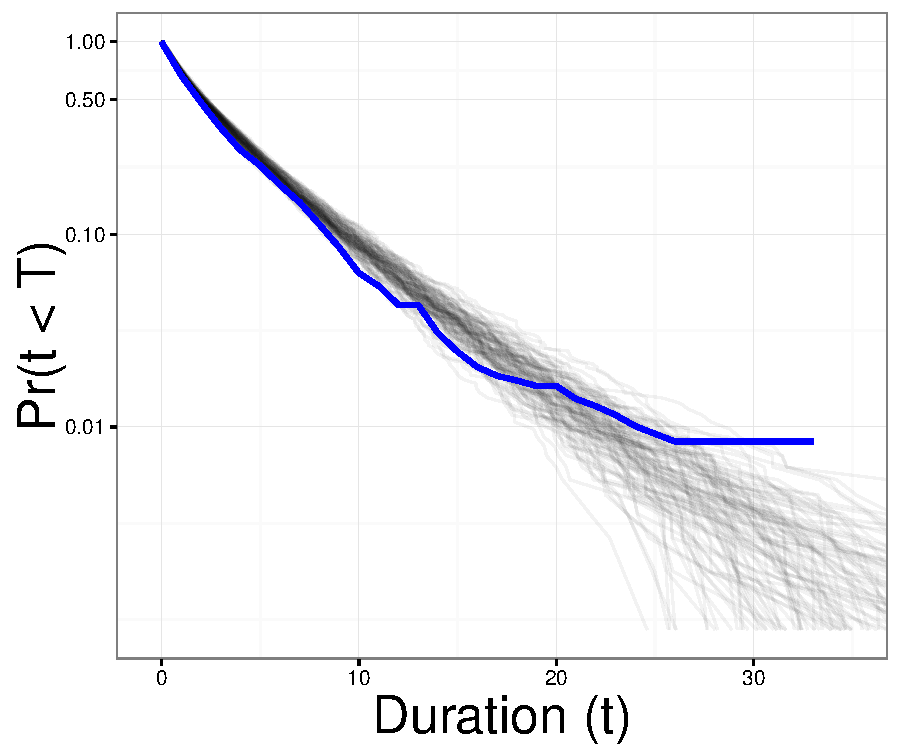
\includegraphics[width=\textwidth,height=0.8\textheight,keepaspectratio=true]{figure/survival_curves}
      \end{center}
    \end{column}
    \begin{column}{0.5\textwidth}
      \begin{center}
        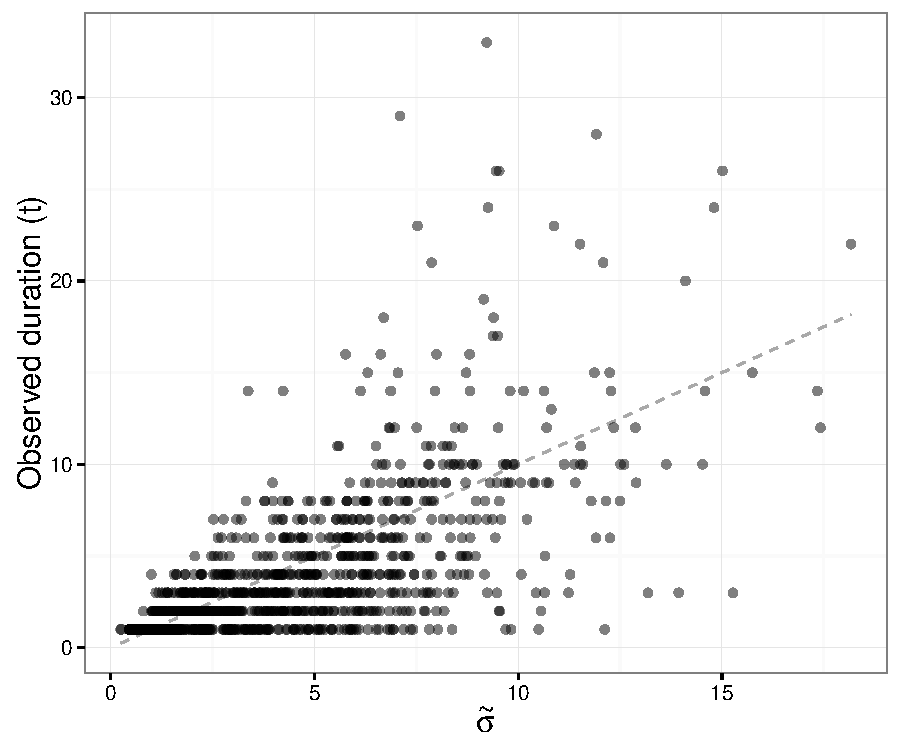
\includegraphics[width=\textwidth,height=0.8\textheight,keepaspectratio=true]{figure/shotgun}
      \end{center}
    \end{column}
  \end{columns}
\end{frame}

\begin{frame}
  \frametitle{Effects of biological traits on survival}
  \begin{center}
    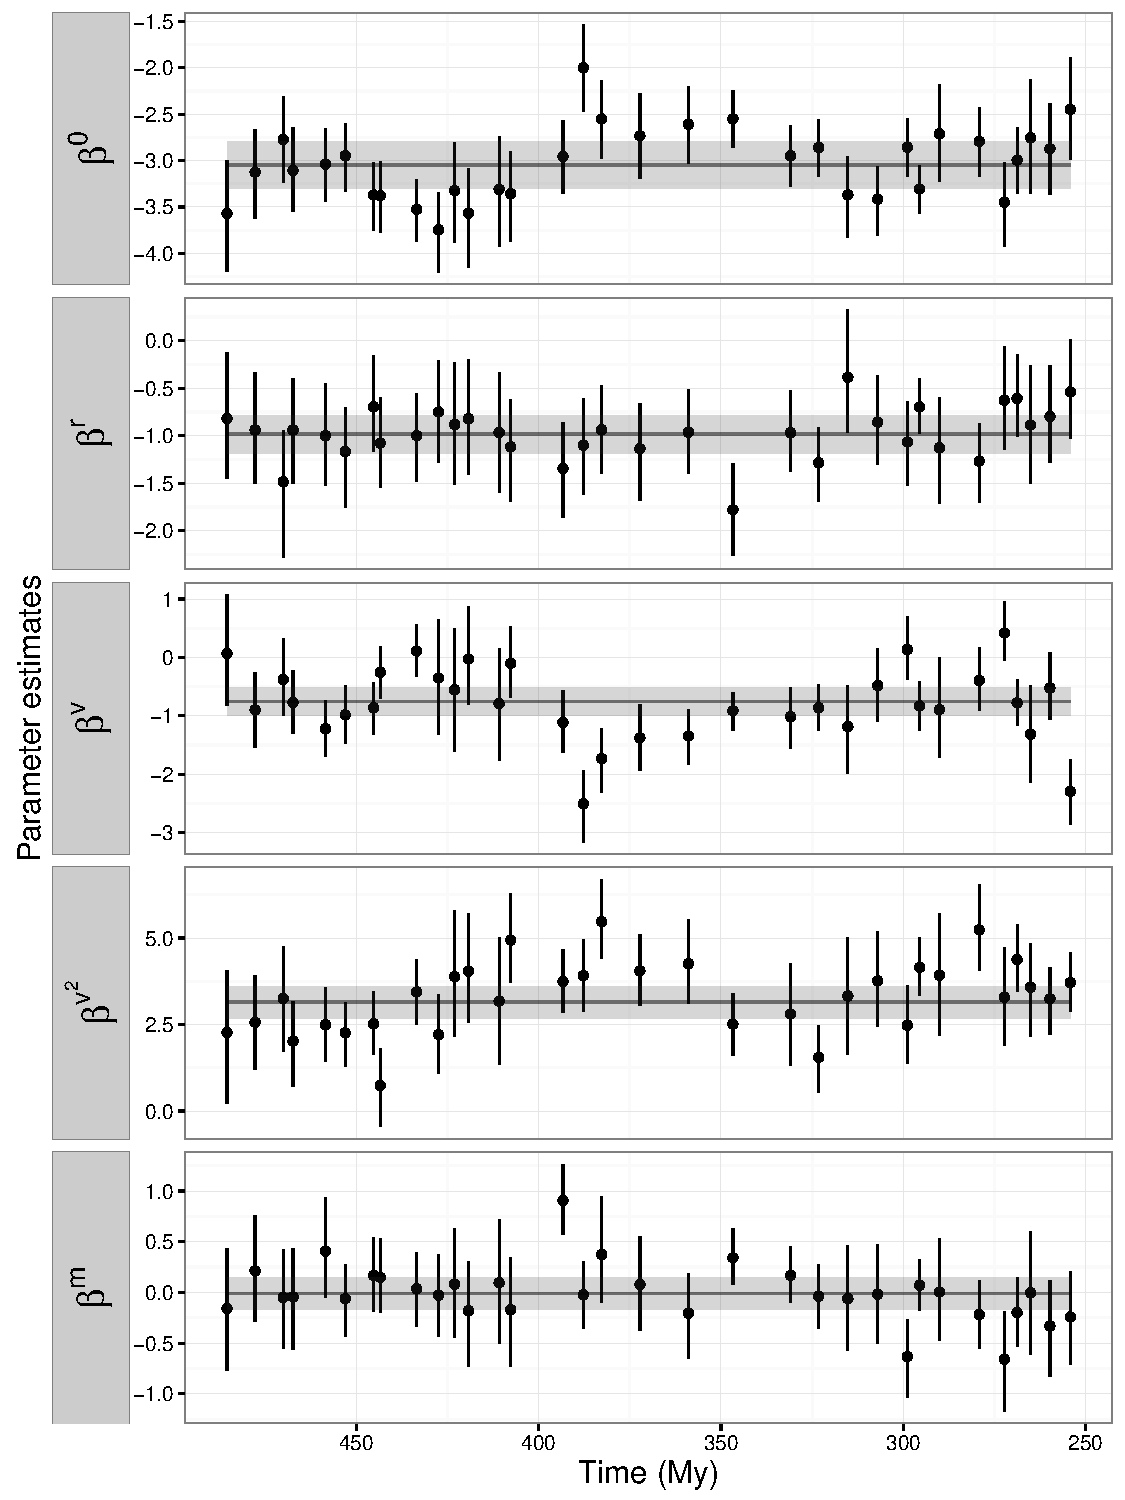
\includegraphics[width=\textwidth,height=0.8\textheight,keepaspectratio=true]{figure/cohort_series}
  \end{center}
\end{frame}

\begin{frame}
  \frametitle{Parabolic effect of environmental preference on survival}
  \begin{center}
    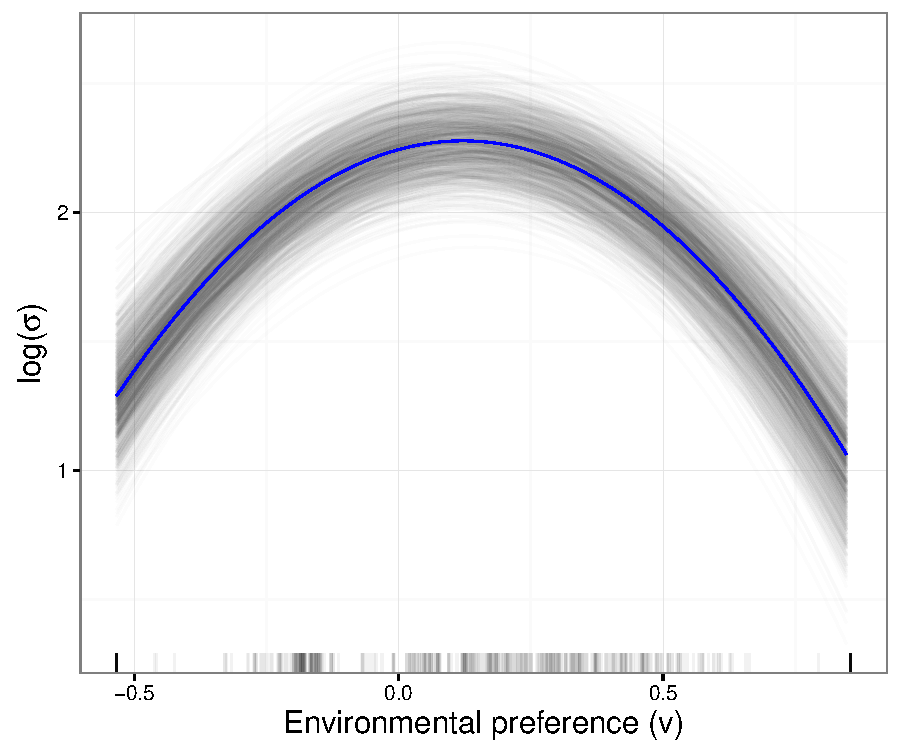
\includegraphics[width=\textwidth,height=0.8\textheight,keepaspectratio=true]{figure/env_effect}
  \end{center}
\end{frame}

\begin{frame}
  \frametitle{Correlation between cohort trait effects}
  \begin{center}
    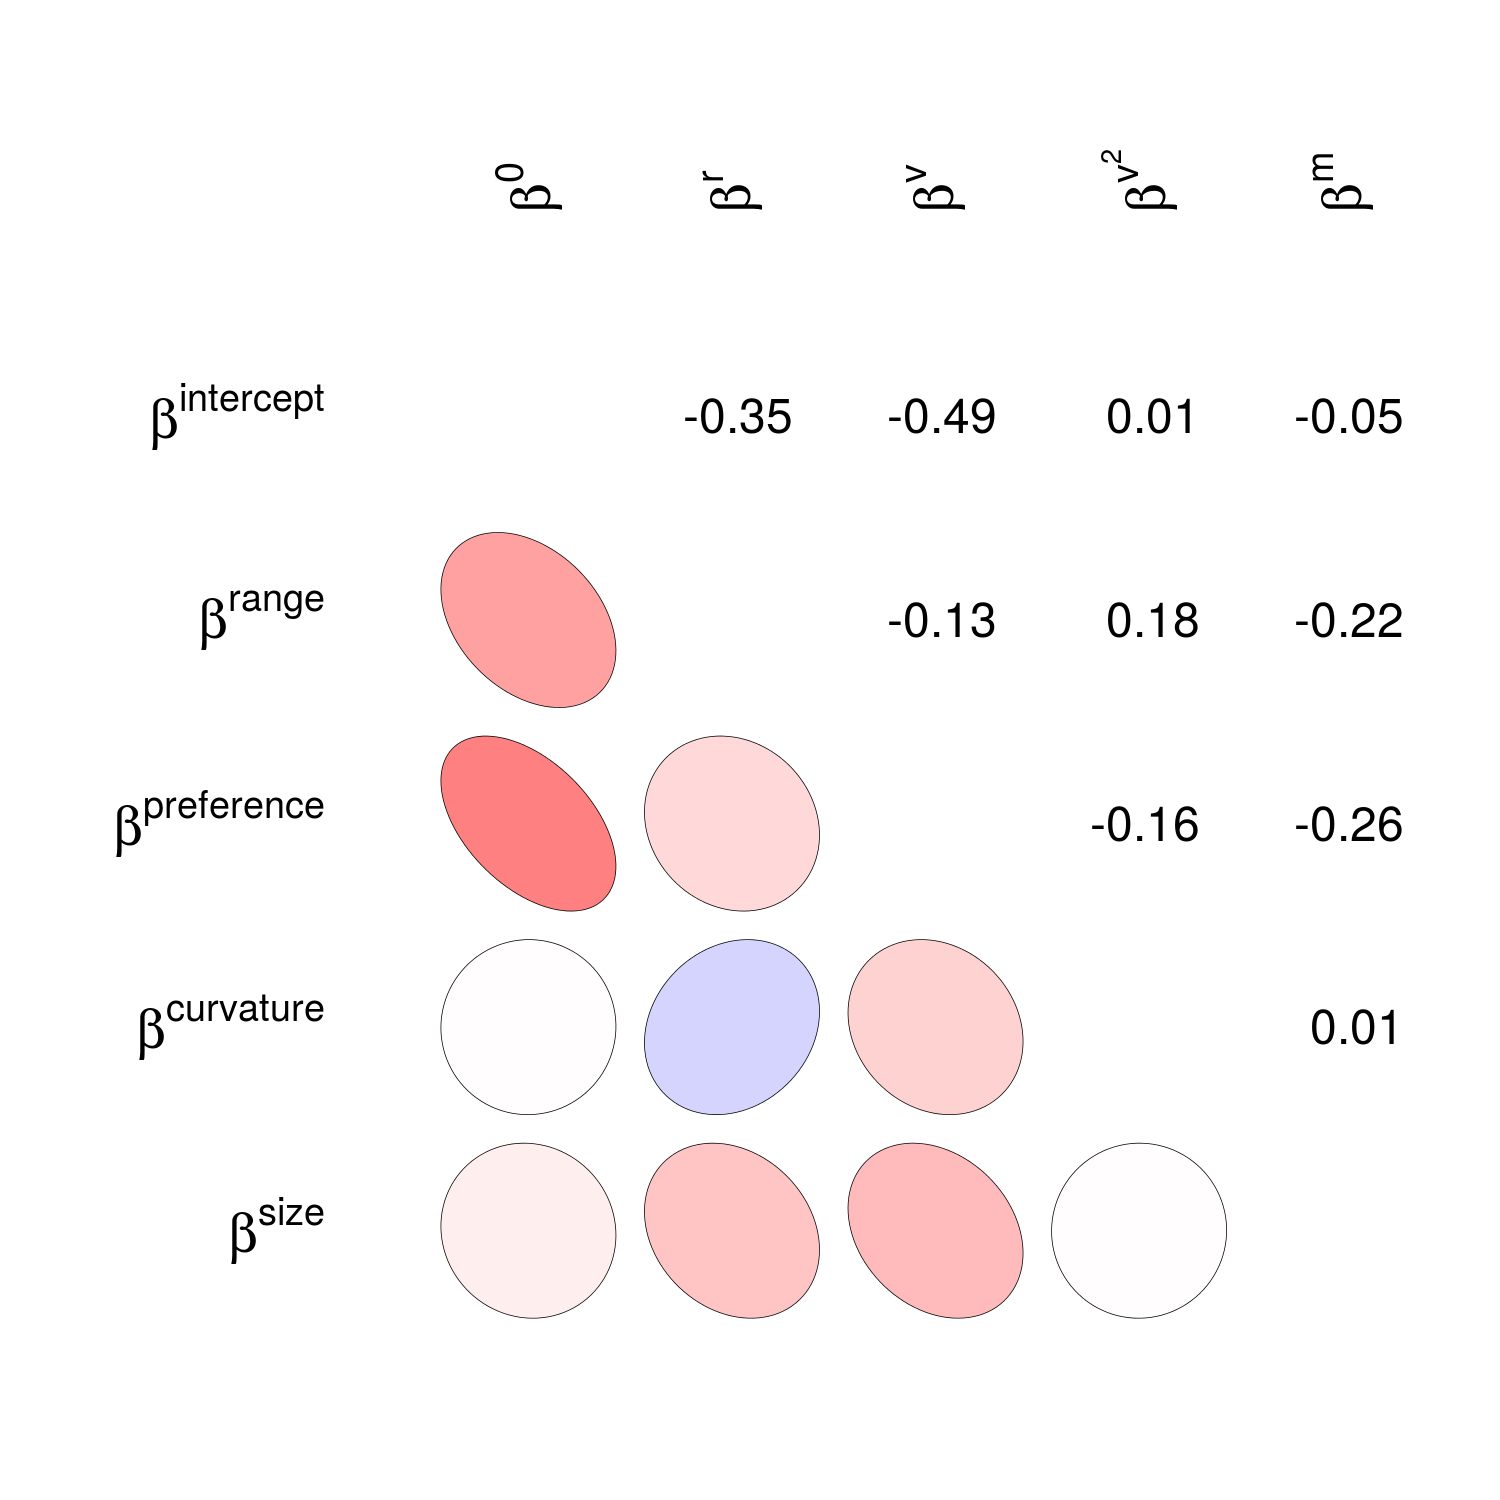
\includegraphics[width=\textwidth,height=0.8\textheight,keepaspectratio=true]{figure/wei_cor_heatmap}
  \end{center}
\end{frame}

\begin{frame}
  \frametitle{Parabolic effect of environmental preference on survival \\by stage}
  \begin{center}
    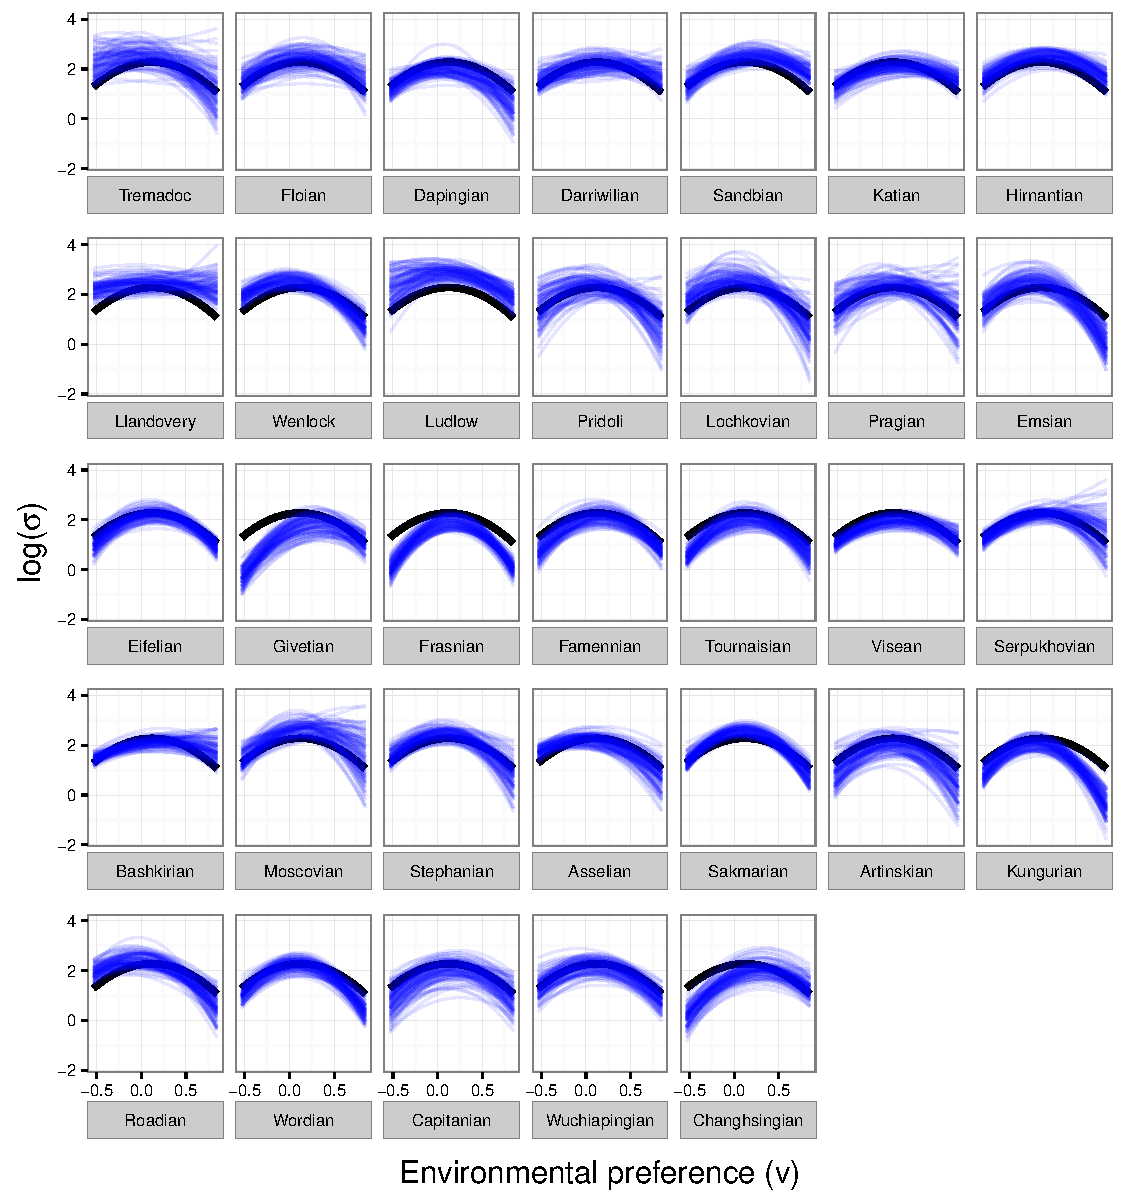
\includegraphics[width=\textwidth,height=0.8\textheight,keepaspectratio=true]{figure/env_cohort}
  \end{center}
\end{frame}

\begin{frame}
  \begin{block}{Conclusions}
    \begin{itemize}
      \item model fit is ok, I wish it was better
      \item strong support for nonlinear relationship between environmental preference and survival
        \begin{itemize}
          \item intermediate preference expected to have greater duration than either end members
        \end{itemize}
      \item correlation between extinction intensity and selectivity
        \begin{itemize}
          \item as average duration increases, effect of geographic range decreases \alert{medium}
          \item as average duration increases, y-intercept of the nonlinear effect of environmental preferences increases (e.g. from slight epicontinental to complete middle) \alert{strong}
        \end{itemize}
      \item increasing extinction risk with taxon age
    \end{itemize}
  \end{block}
\end{frame}

\begin{frame}
  \begin{alertblock}{Updates}
    \begin{itemize}
      \item presented at GSA 2015
      \item rejected from \textit{Evolution}
        \begin{itemize}
          \item encouraged resubmit
          \item audience issues
          \item difficult but transformational reviews
          \item resubmitted 3 March
          \item still ``under review'' as of this morning (70 days)
        \end{itemize}
    \end{itemize}
  \end{alertblock}
\end{frame}



\section{Taxon occurrence as a function of both emergent biological traits and environmental context}

\begin{frame}
  \frametitle{Initial empirical setup}
  \begin{itemize}
    \item arboreal taxa are expected to have greatest extinction risk of the locomotor categories (Smits 2015 PNAS)
    \item two possible causes
      \begin{enumerate}
        \item this effect is constant for all time
        \item Paleogene-Neogene transition
          \begin{itemize}
            \item neutral effect of arboreality during Paleogene
            \item strong selection against arboreality during Neogene
            \item Neogene effect is stronger than Paleogene effect
            \item means that overall mean effect is closer to Neogene
          \end{itemize}
      \end{enumerate}
    \item former implies no appreciable demographic differences \\over Cenozoic
    \item latter implies a difference in demography between \\Paleogene and Neogene
  \end{itemize}
\end{frame}

\begin{frame}
  \begin{block}{The ground-dwelling problem}
    \begin{itemize}
      \item ``ground-dwelling'' too broad a category
      \item following a suggestion from Graham, split by foot posture
        \begin{itemize}
          \item based primarily on Carrano 1997 \textit{ZJLS}
        \end{itemize}
      \item allows for estimation of subtler shifts in demography \\within ``ground-dwelling''
    \end{itemize}
  \end{block}
\end{frame}

\begin{frame}
  \frametitle{Other covariates of interest}
  \begin{itemize}
    \item traits
      \begin{itemize}
        \item dietary category (shifts in trophic structure)
        \item body mass
      \end{itemize}
    \item environmental factors
      \begin{itemize}
        \item floral phase following Graham 2010 \underline{A Natural History of the New World}
        \item global temperature, both mean and interquartile range
      \end{itemize}
  \end{itemize}

  \begin{block}{traits vary with time; \\environmental factors predict average occurrence probability}
    can estimate probability of expected enrichment or depletion effect of individual traits for each time bin wrt all other analyzed traits
  \end{block}
\end{frame}

\begin{frame}
  \begin{block}{Theoretical underpinning}
    \begin{itemize}
      \item changes in demographic structure of regional species pool
        \begin{itemize}
          \item I'm not modeling the diversification process, \alert{only presence}
          \item no difference between origination, survival, extinction in effect
        \end{itemize}
      \item intersection of macroecology and macroevolution
      \item fourth-corner type problem
        \begin{itemize}
          \item trait- \textbf{and} environment-based assembly
        \end{itemize}
    \end{itemize}
  \end{block}
\end{frame}

\begin{frame}
  \frametitle{Conceptual diagram of fourth-corner problem}

  \begin{center}
    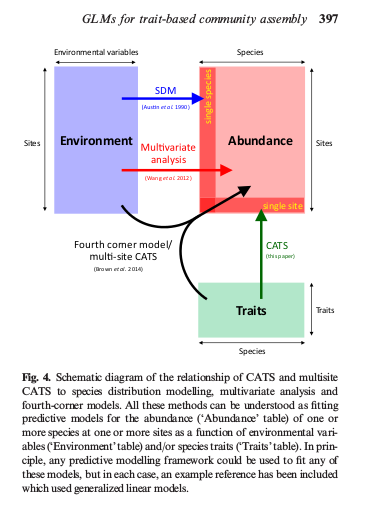
\includegraphics[width=\textwidth,height=0.7\textheight,keepaspectratio=true]{figure/warton_4corner}
  \end{center}

  \attrib{\scriptsize{Warton, Shipley, and Hastie. 2015. \textit{Methods in Ecology and Evolution.}}}
\end{frame}

\begin{frame}
  \frametitle{Conceptual diagram of my model}
  \begin{center}
    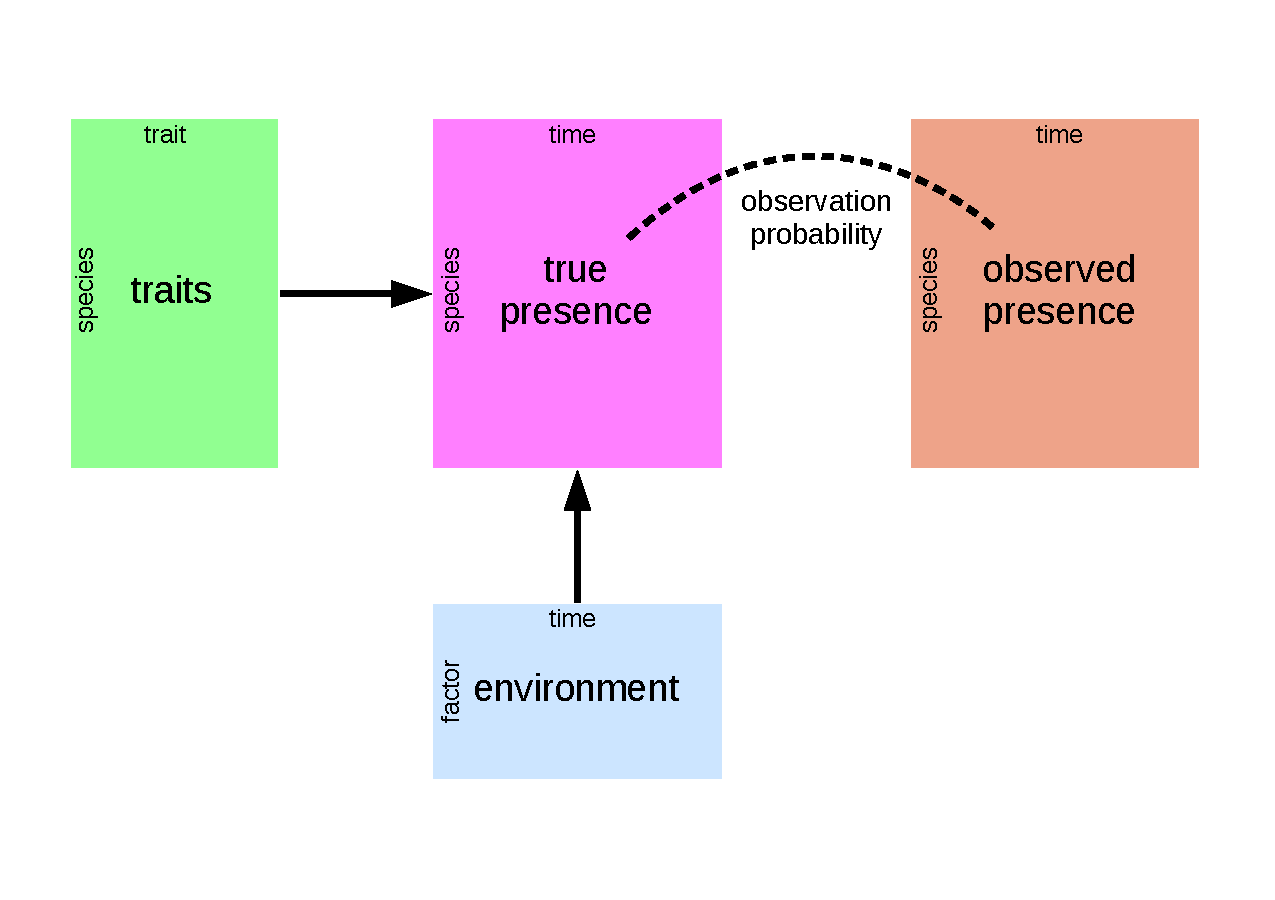
\includegraphics[width=\textwidth,height=0.8\textheight,keepaspectratio=true]{figure/paleo_fourth_corner}
  \end{center}
\end{frame}

\begin{frame}
  \frametitle{Analysis of Cenozoic mammal fossil record for NA}
  \begin{columns}
    \begin{column}{0.5\textwidth}
      individual-level \\(genus i at time unit t)
      \begin{itemize}
        \item log-odds of occurrence probability at time t
        \item effect of locomotor type
          \begin{itemize}
            \item arboreal, digitigrade, plantigrade, unguligrade, fossorial, scansorial
          \end{itemize}
        \item effect of dietary type
          \begin{itemize}
            \item carnivore, herbivore, insectivore, omnivore
          \end{itemize}
        \item effect body size \\(rescaled log body mass)
      \end{itemize}
    \end{column}
    \begin{column}{0.5\textwidth}
      group-level (2 My time unit t)
      \begin{itemize}
        \item overall mean of log-odds of occurrence probability
        \item temperature record based on Mg/Ca estimates
          \begin{itemize}
            \item mean and interquartile range of rescaled value
          \end{itemize}
        \item plant community phase following Graham
      \end{itemize}
    \end{column}
  \end{columns}
\end{frame}


\begin{frame}
  \frametitle{Model of taxon occurrence}
  \begin{itemize}
    \item response is p/a of genus in NA at time \(t\)
      \begin{itemize}
        \item Bernoulli variable 
        \item probability is (observation prob) times (``true'' presence)
      \end{itemize}
    \item observation probability is effect of sampling/fossil record
    \item the latent discrete ``true'' presence modeled as a \\multi-level logistic regression
      \begin{itemize}
        \item individual- and group-level
      \end{itemize}
  \end{itemize}
\end{frame}

\begin{frame}
  \frametitle{Sampling statement for the joint posterior probability}
  \footnotesize{
    \begin{align*}
      y_{i,t} &\sim \text{Bernoulli}(\rho_{t} z_{i,t}) \\
      \text{logit}(\rho_{t}) &\sim \mathcal{N}(\rho^{'}, \sigma_{\rho}) \\
      z_{i,t} &\sim \text{Bernoulli}(\theta_{i, t}) \\
      \text{logit}(\theta_{i, t}) &= z_{i,t-1} (\alpha_{t} + X_{i} \beta_{t\_}) + (\prod_{k = 1}^{t-1} 1 - z_{i,k}) (\alpha_{t} + X_{i} \beta_{t\_}) \\
      \beta_{t,d} &\sim \mathcal{N}(\mu_{d}, \sigma_{d}) \\
      \alpha_{t} &\sim \mathcal{N}(\mu + \phi_{p[t]} + U_{t} \gamma, \sigma_{\mu}) \\
      \phi_{p} &\sim \mathcal{N}(0, \sigma_{\phi}) \\
    \end{align*}
  }
  \scriptsize{Note: Product term ensures taxon-loss is permanent. Implementation in Stan marginalizes over all possible (range-through) values of \(z\) instead of estimating the discrete parameters. I also use a noncentered parameterization of the hierarchical effects for better posterior sampling behavior. This presentation excludes final (hyper)priors.}
\end{frame}

\begin{frame}
  \begin{block}{Assessing model fit from the posterior predictive distribution}
    \begin{itemize}
      \item simulate fossil record given only \(y_{\_t = 1}\) given all covariates, \(\theta\)
        \begin{itemize}
          \item where \(\theta\) is the set of all parameters
        \end{itemize}
      \item cross-validation for time series
        \begin{itemize}
          \item Bayesian statement is \(p(\tilde{y}_{\_(t + 1)} | y_{\_t}, \theta)\)
          \item issues because of high structured data (e.g. floral phase)
        \end{itemize}
    \end{itemize}
  \end{block}
\end{frame}

\begin{frame}
  \begin{alertblock}{Current project issues}
    \begin{itemize}
      \item fit with Stan (NUTS sampling/MCMC of posterior)
      \item crocorock CEB server
      \item 4 parallel chains
        \begin{itemize}
          \item 10 000 warm-up, 10 000 sampling, thinned by 10
        \end{itemize}
      \item slow to converge 
        \begin{itemize}
          \item simple model with no individual- or group-level effects \\takes a week (same settings)
        \end{itemize}
      \item solutions?
        \begin{itemize}
          \item restrict taxonomic or temporal scope?
          \item decrease model complexity: where and how?
          \item other reparameterizations?
        \end{itemize}
    \end{itemize}
  \end{alertblock}
\end{frame}


\section{Collaboration projects}

\begin{frame}
  \frametitle{How cryptic is cryptic diversity? Machine learning approaches to classifying morphological variation in the Pacific Pond Turtle (\textit{Emys marmorata})}
  \begin{itemize}
    \item estimate which species classification is best supported by morphology
      \begin{itemize}
        \item multiple machine learning approaches
        \item three datasets; special attention to \textit{Emys}
        \item comparison of in- and out-of-sample model performance
      \end{itemize}
    \item collaboration with Ken, Jim Parham, and Bryan Stuart
    \item submitted to then rejected from Systematic Biology
  \end{itemize}
\end{frame}

\begin{frame}
  \begin{block}{Statistical learning approach}
    \begin{itemize}
      \item split data into training and testing datasets (80/20)
      \item training dataset
        \begin{itemize}
          \item multiple models w/ between 3-28 predictors
          \item 10 rounds, 5-fold cross-validation
            \begin{itemize}
              \item estimate out-of-sample AUC of ROC
              \item compare for model selection 
            \end{itemize}
          \item follows Hastie et al. 2009 ``Elements of Statistical Learning''
        \end{itemize}
      \item testing dataset
        \begin{itemize}
          \item using selected model, predict classification
          \item AUC of ROC as measure of success
          \item compare average from multiple models to compare hypotheses
        \end{itemize}
    \end{itemize}
  \end{block}
\end{frame}

\begin{frame}
  \frametitle{PC-s for the 7 turtle and \textit{Trachemys} species sets}
  \begin{center}
    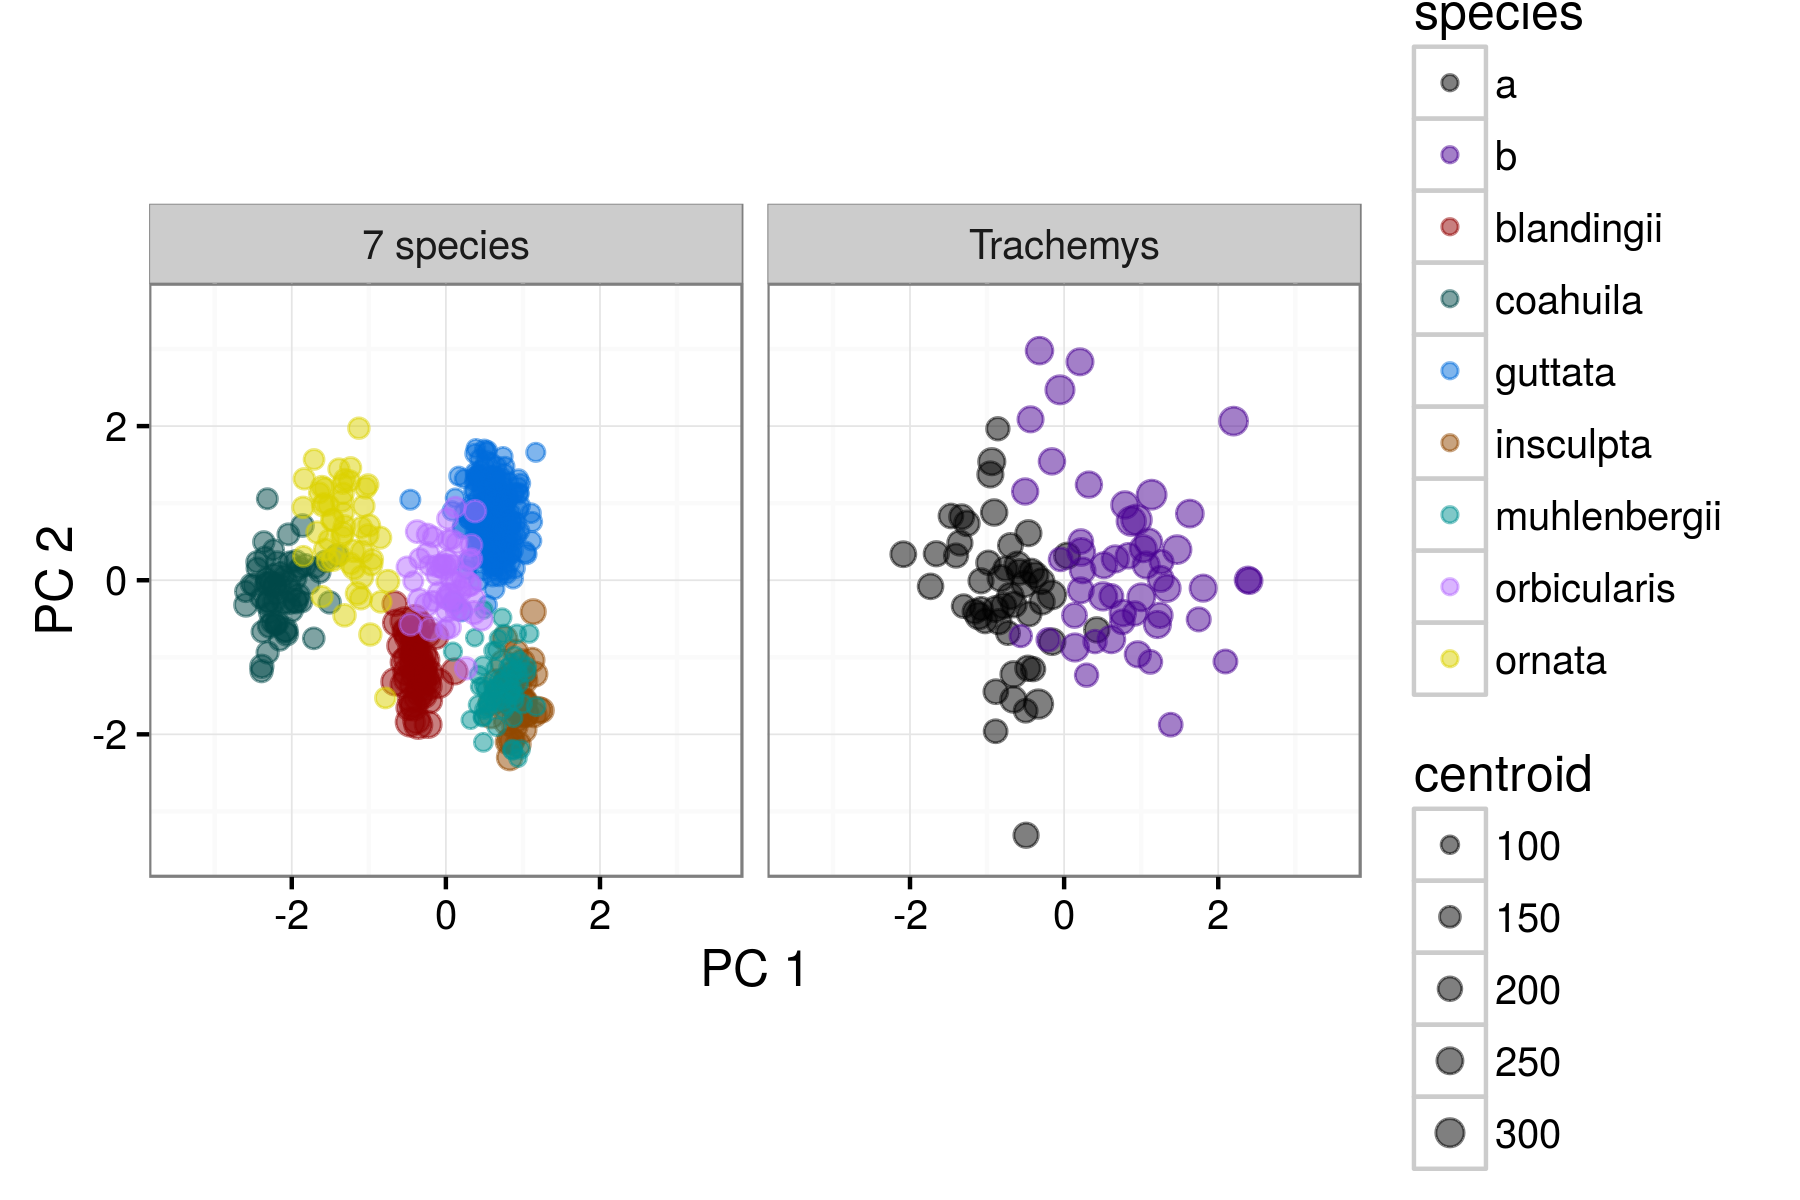
\includegraphics[width=\textwidth,height=0.8\textheight,keepaspectratio=true]{figure/other_pc_graph}
  \end{center}
\end{frame}

\begin{frame}
  \frametitle{7 turtle, and \textit{Trachemys} species sets}
  \begin{columns}
    \begin{column}{0.5\textwidth}
      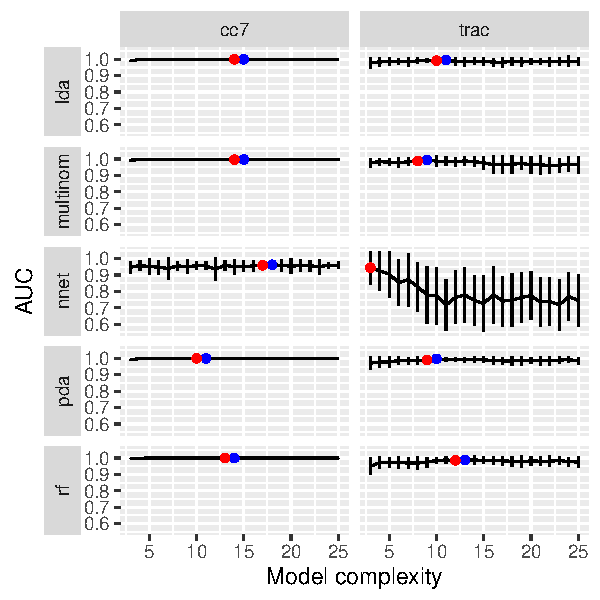
\includegraphics[width=\textwidth,height=0.8\textheight,keepaspectratio=true]{figure/other_model_sel}
    \end{column}
    \begin{column}{0.5\textwidth}
      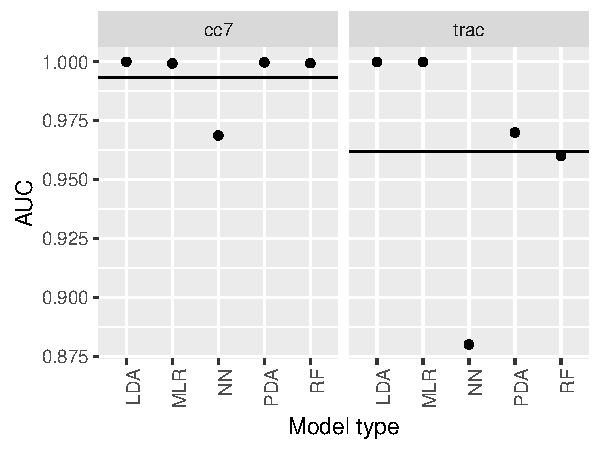
\includegraphics[width=\textwidth,height=0.8\textheight,keepaspectratio=true]{figure/other_oos_sel}
    \end{column}
  \end{columns}
\end{frame}

\begin{frame}
  \frametitle{PC-s for the \textit{Emys} species sets}
  \begin{center}
    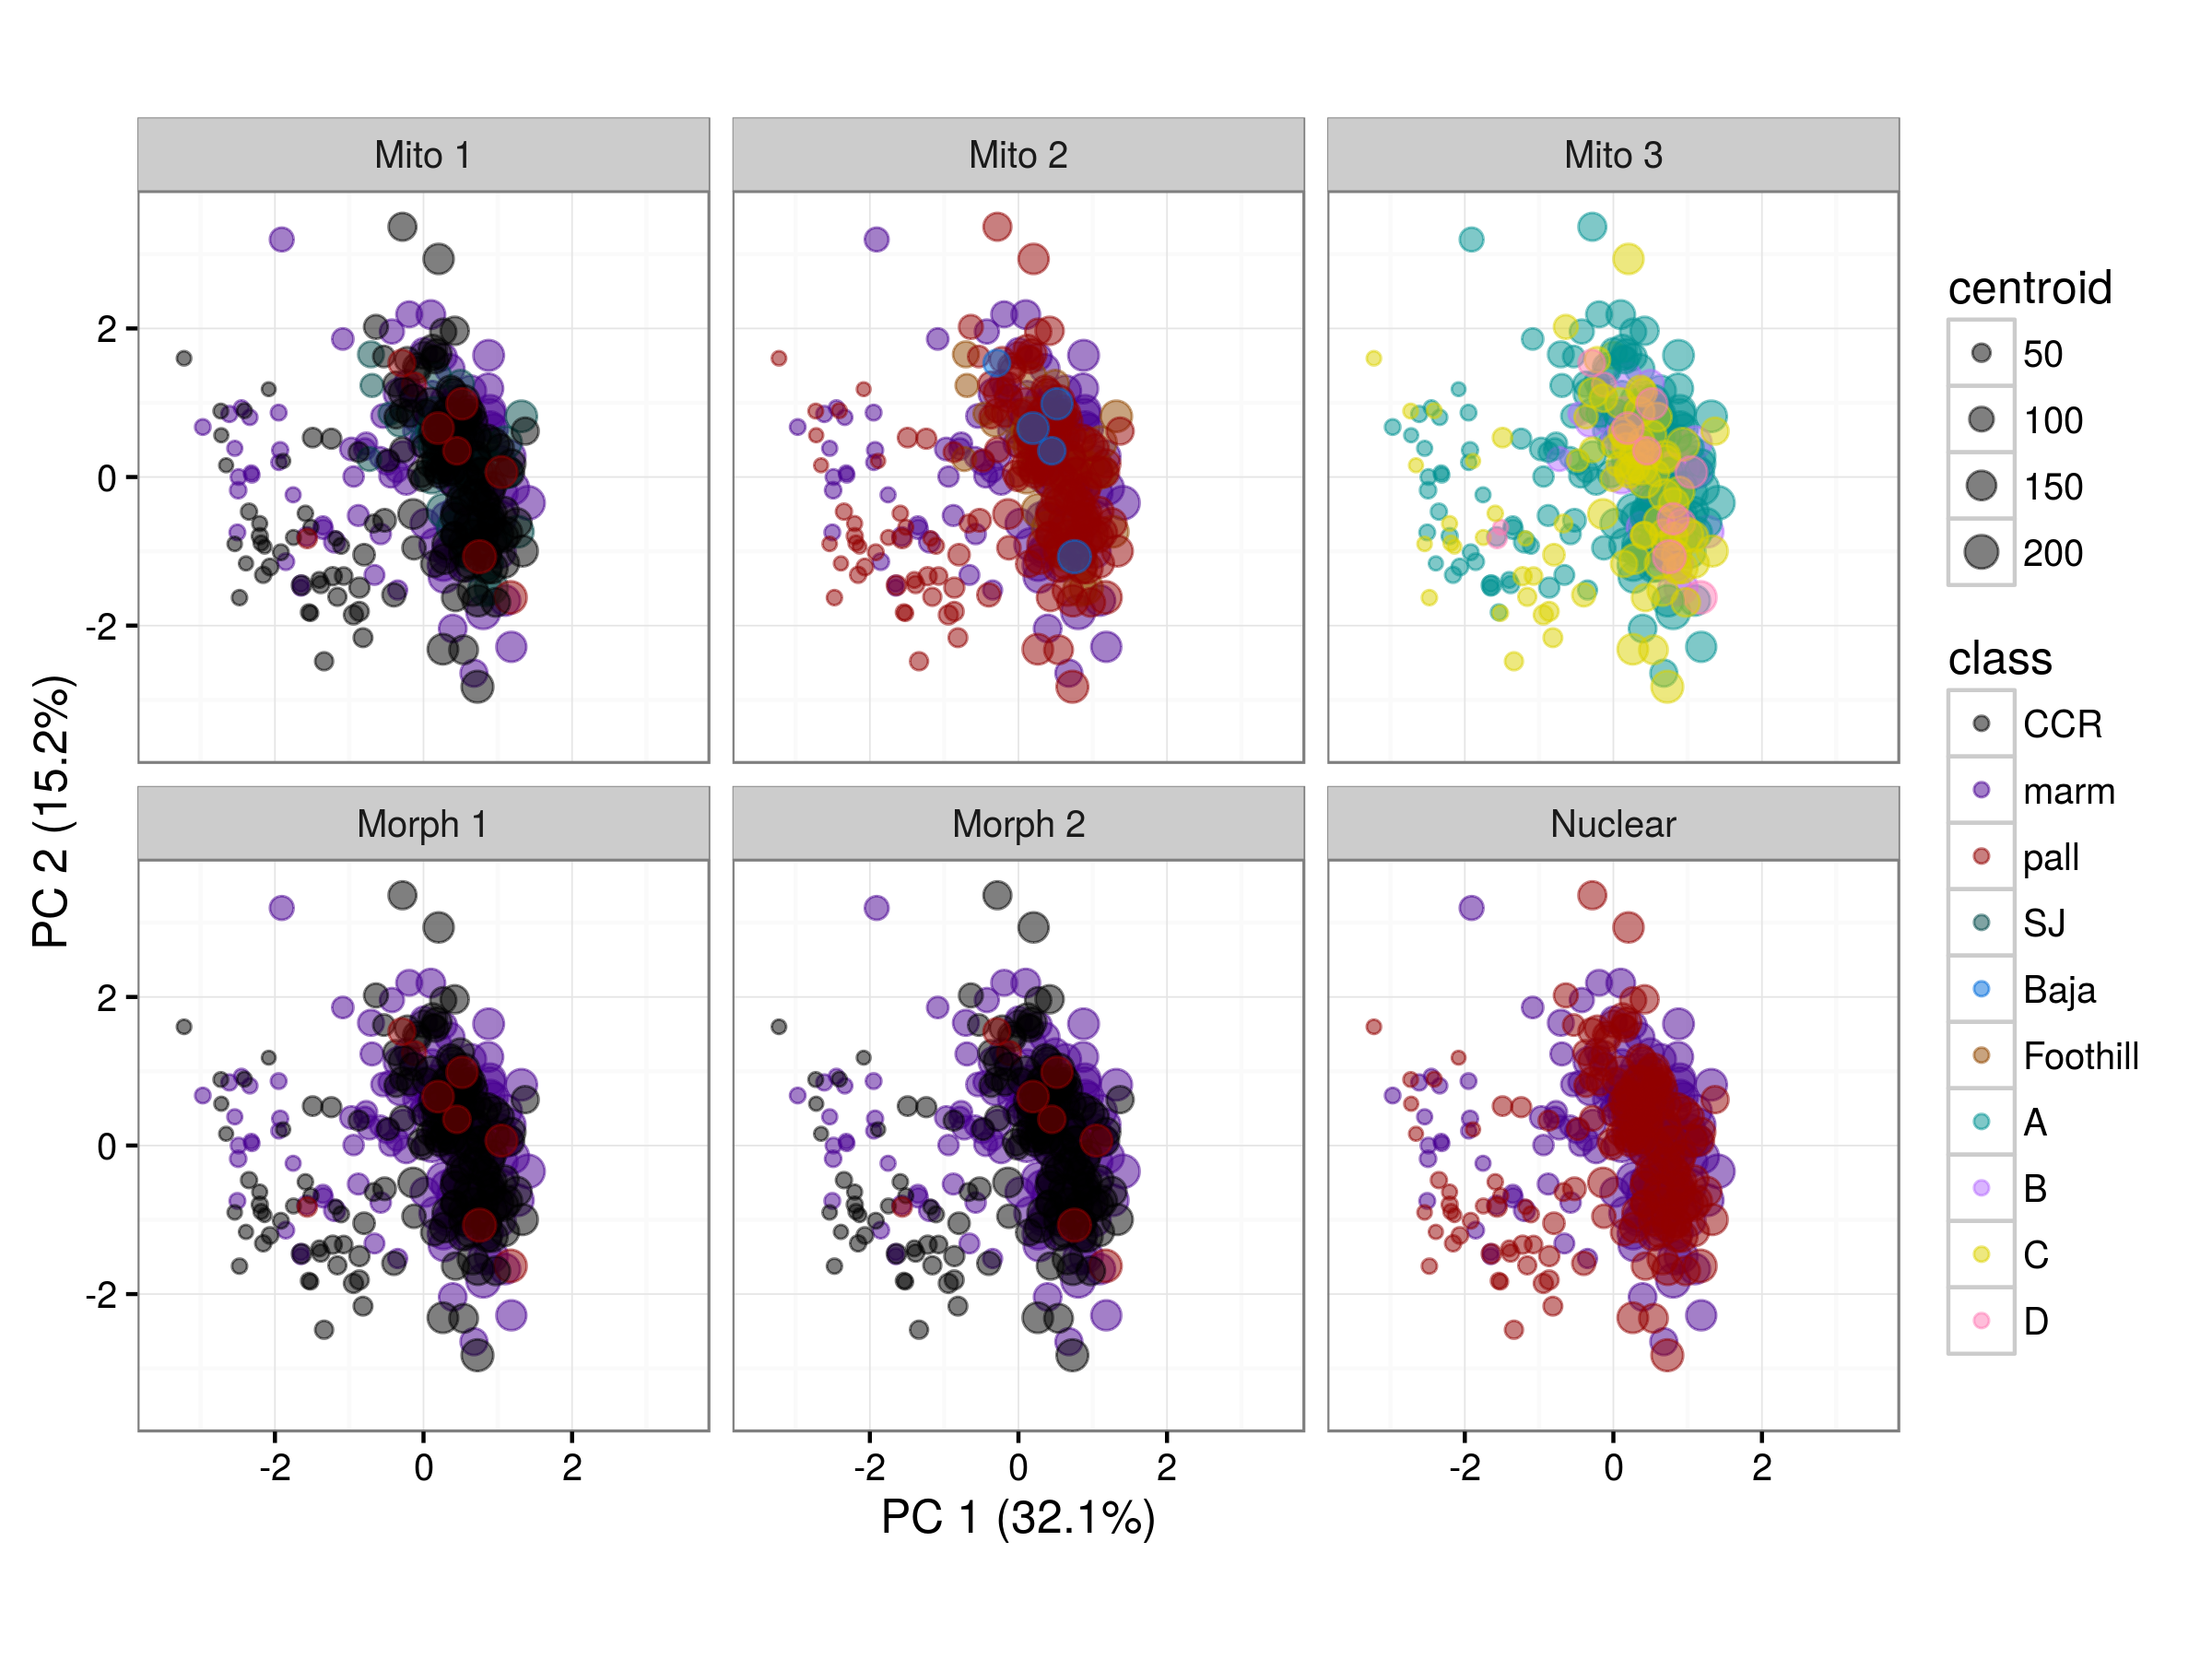
\includegraphics[width=\textwidth,height=0.8\textheight,keepaspectratio=true]{figure/emys_pc_graph}
  \end{center}
\end{frame}

\begin{frame}
  \frametitle{\textit{Emys}: CV of model using training data}
  \begin{center}
    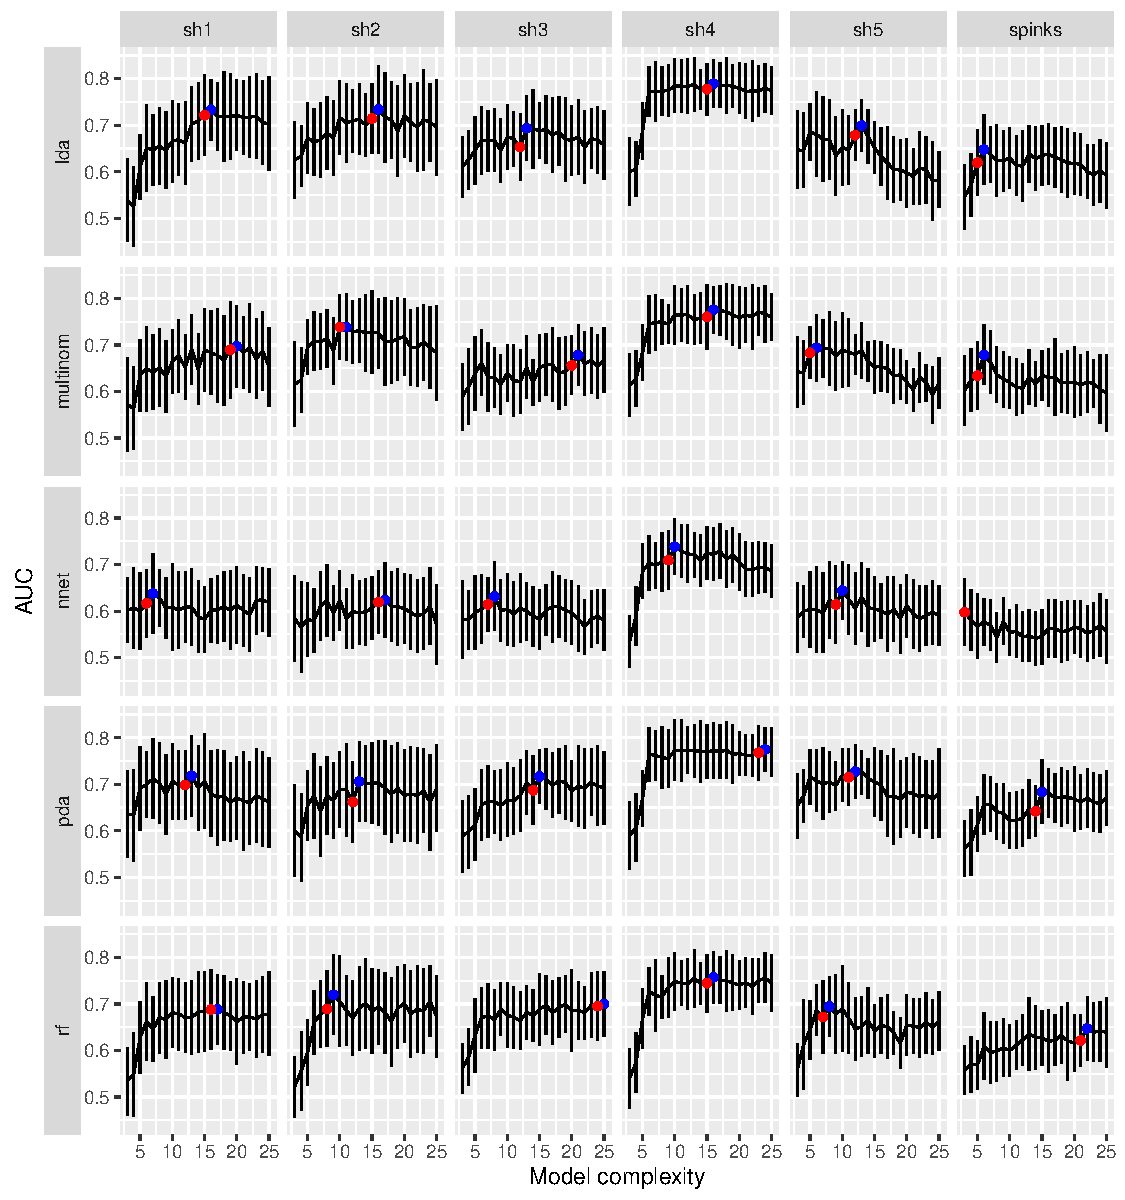
\includegraphics[width=\textwidth,height=0.8\textheight,keepaspectratio=true]{figure/emys_model_sel}
  \end{center}
\end{frame}

\begin{frame}
  \frametitle{\textit{Emys}: Results of prediction of testing data}
  \begin{center}
    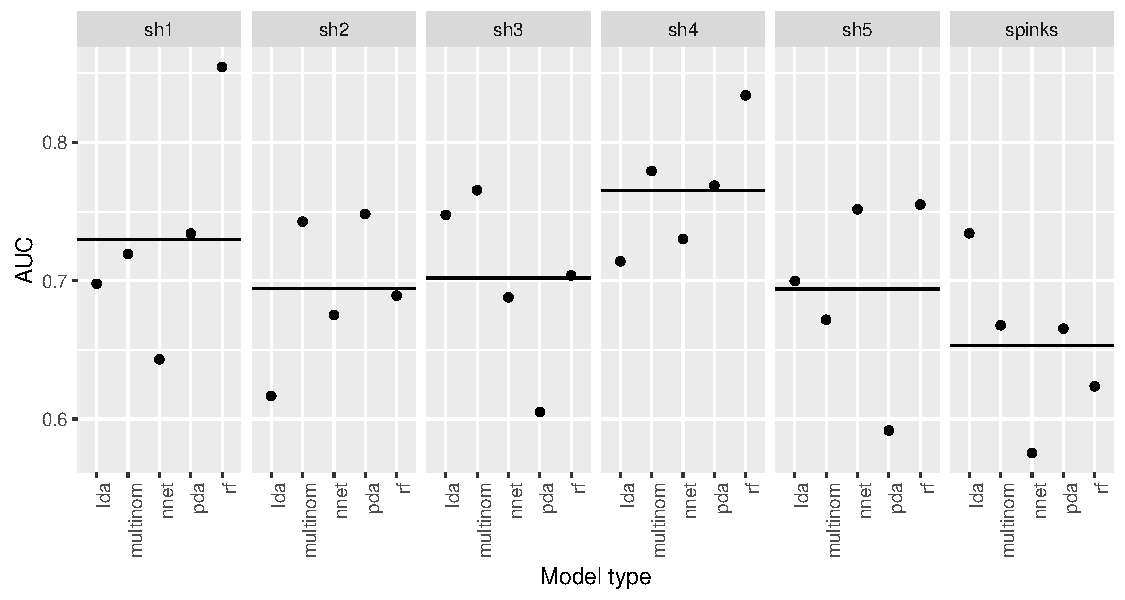
\includegraphics[width=\textwidth,height=0.8\textheight,keepaspectratio=true]{figure/emys_oos_sel}
  \end{center}
\end{frame}


% bivalve naming rate w/ stewart
\begin{frame}
  \frametitle{Modeling the rate at which new species are named.}

  \begin{block}{Goal}
    Predictive model of number of bivalve species named (per publication) per year by biogeographic province.
  \end{block}

  \begin{columns}
    \begin{column}{0.5\textwidth}
      \begin{itemize}
        \item collaboration with Stewart Edie
        \item he developed the question, \\I developed the model
      \end{itemize}
    \end{column}
    \begin{column}{0.5\textwidth}
      \begin{itemize}
        \item hierarchical zero-inflated Poisson time-series model
        \item forecast rank order of provincial diversity in approx. 15 years
      \end{itemize}
    \end{column}
  \end{columns}
\end{frame}

\begin{frame}
  \frametitle{Conceptual model}
  \begin{center}
    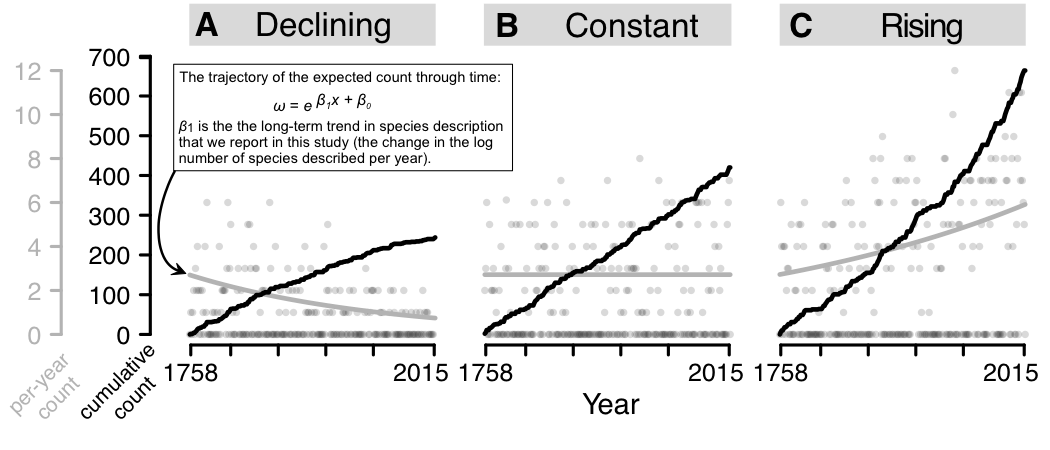
\includegraphics[width=\textwidth,height=0.8\textheight,keepaspectratio=true]{figure/edie_concept}
  \end{center}

  \attrib{\scriptsize{Edie, Smits, et al. \textit{in. prep.}}}
\end{frame}

\begin{frame}
  \frametitle{Regional accumulation and prior predictive comparison}

  \begin{center}
    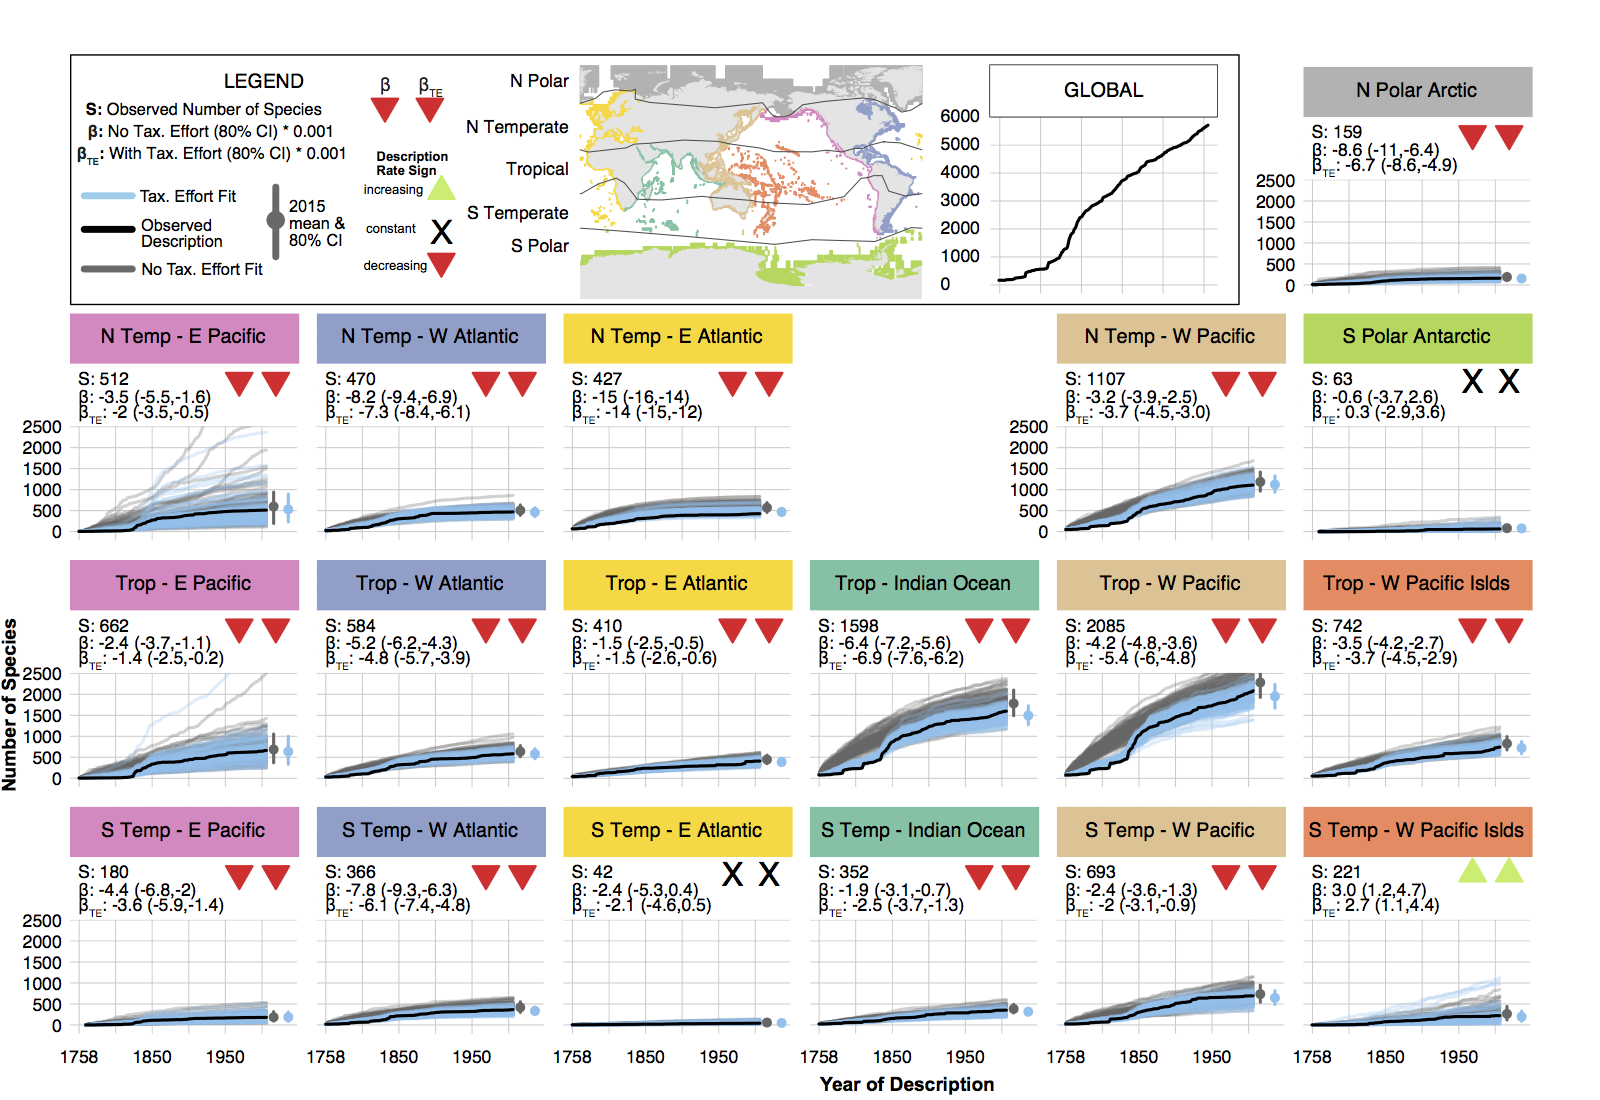
\includegraphics[width=\textwidth,height=0.8\textheight,keepaspectratio=true]{figure/edie_cumm_regional}
  \end{center}

  \attrib{\scriptsize{Edie, Smits, et al. \textit{in. prep.}}}
\end{frame}

\begin{frame}
  \frametitle{Cross-validation of forecasting error}

  \begin{center}
    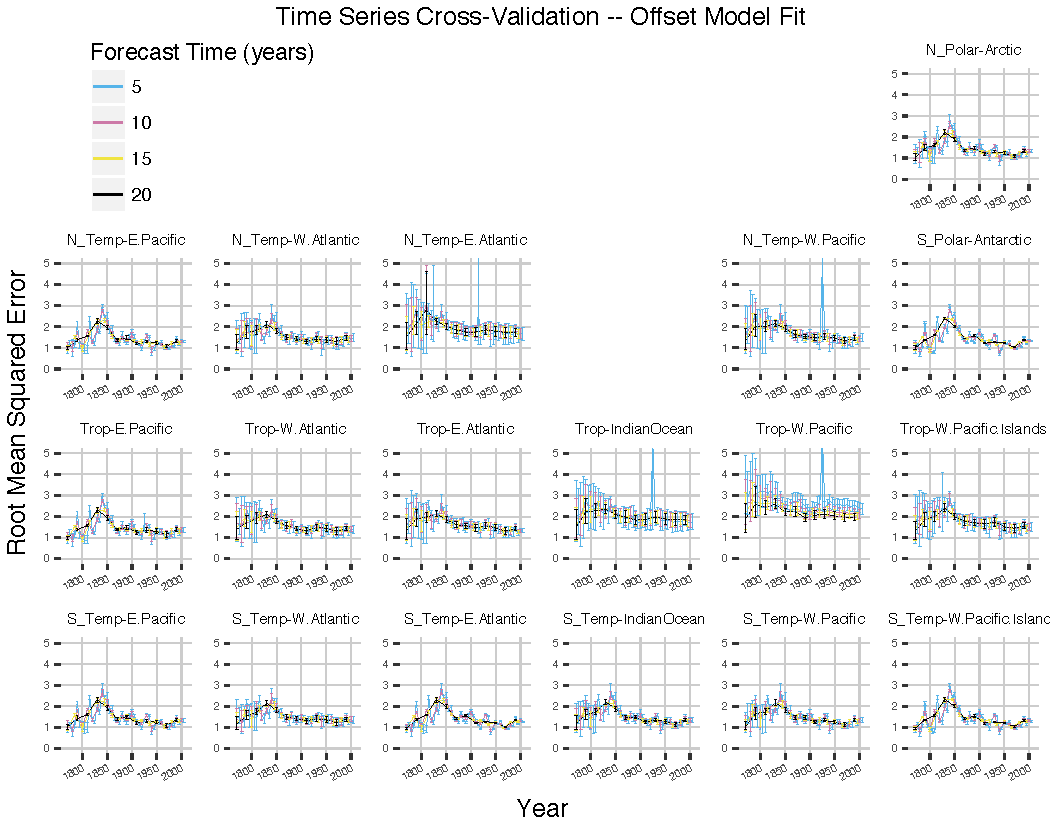
\includegraphics[width=\textwidth,height=0.8\textheight,keepaspectratio=true]{figure/edie_cv_forecast}
  \end{center}

  \attrib{\scriptsize{Edie, Smits, et al. \textit{in. prep.}}}
\end{frame}

\begin{frame}
  \frametitle{Forecasted regional ranks}

  \begin{center}
    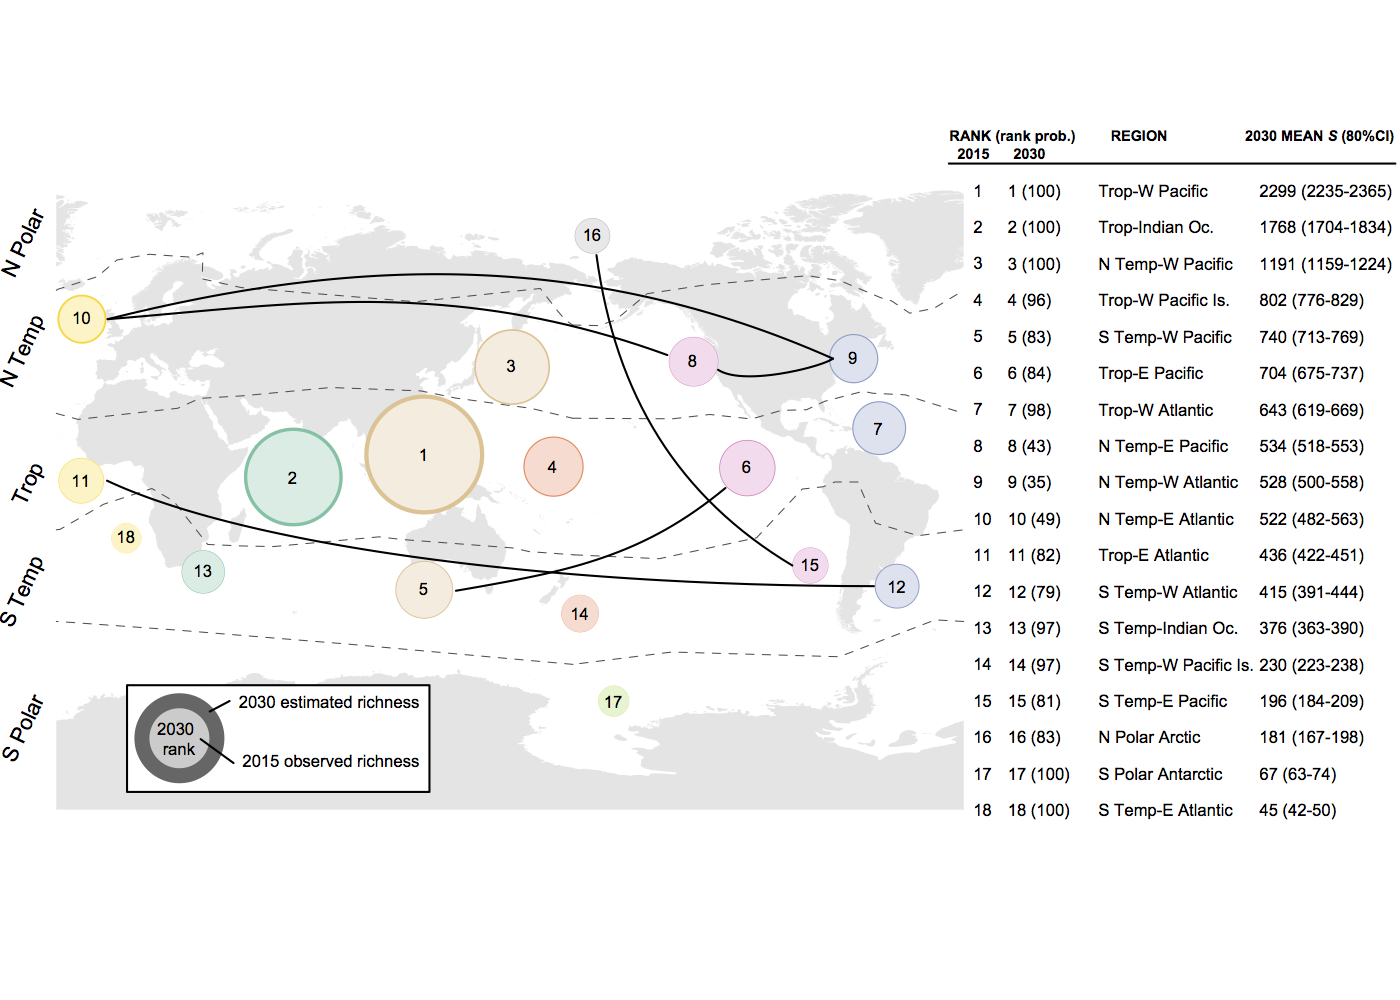
\includegraphics[width=\textwidth,height=0.8\textheight,keepaspectratio=true]{figure/edie_rank}
  \end{center}

  \attrib{\scriptsize{Edie, Smits, et al. \textit{in. prep.}}}
\end{frame}


\section{Moving forward}

\begin{frame}
  \frametitle{people to post-doc with and related fellowships}
  \begin{enumerate}
    \item \textbf{Miller Fellowship at Berkeley with Charles Marshall}
      \begin{itemize}
        \item Charles has met me a couple times.
      \end{itemize}
    \item \textbf{Peter Buck Fellowship at Smithsonian with Gene Hunt \\(and Peter Wagner and Kate Lyons)}
      \begin{itemize}
        \item Gene, Pete, and Kate all know who I am.
      \end{itemize}
    \item \textbf{Michigan Fellowship at University of Michigan \\with Matt Friedman}
      \begin{itemize}
        \item I don't know him
      \end{itemize}
    \item \textbf{NIMBiOS Post-doc with Brian O'Meara}
      \begin{itemize}
        \item I don't know him.
      \end{itemize}
  \end{enumerate}
\end{frame}


\begin{frame}
  \begin{block}{My ``research program''}
    \begin{itemize}
      \item macroevolutionary macroecology
        \begin{itemize}
          \item research at the intersection of disciplines
        \end{itemize}
      \item hypothesis driven
        \begin{itemize}
          \item empirical tests of macroevolutionary theories
        \end{itemize}
      \item modeling (Bayesian, hierarchical/GLMM)
        \begin{itemize}
          \item emphasis on model checking and validation
        \end{itemize}
    \end{itemize}
  \end{block}
\end{frame}



\end{document}
